\documentclass{article}\usepackage[]{graphicx}\usepackage[]{color}
%% maxwidth is the original width if it is less than linewidth
%% otherwise use linewidth (to make sure the graphics do not exceed the margin)
\makeatletter
\def\maxwidth{ %
  \ifdim\Gin@nat@width>\linewidth
    \linewidth
  \else
    \Gin@nat@width
  \fi
}
\makeatother

\definecolor{fgcolor}{rgb}{0.345, 0.345, 0.345}
\newcommand{\hlnum}[1]{\textcolor[rgb]{0.686,0.059,0.569}{#1}}%
\newcommand{\hlstr}[1]{\textcolor[rgb]{0.192,0.494,0.8}{#1}}%
\newcommand{\hlcom}[1]{\textcolor[rgb]{0.678,0.584,0.686}{\textit{#1}}}%
\newcommand{\hlopt}[1]{\textcolor[rgb]{0,0,0}{#1}}%
\newcommand{\hlstd}[1]{\textcolor[rgb]{0.345,0.345,0.345}{#1}}%
\newcommand{\hlkwa}[1]{\textcolor[rgb]{0.161,0.373,0.58}{\textbf{#1}}}%
\newcommand{\hlkwb}[1]{\textcolor[rgb]{0.69,0.353,0.396}{#1}}%
\newcommand{\hlkwc}[1]{\textcolor[rgb]{0.333,0.667,0.333}{#1}}%
\newcommand{\hlkwd}[1]{\textcolor[rgb]{0.737,0.353,0.396}{\textbf{#1}}}%

\usepackage{framed}
\makeatletter
\newenvironment{kframe}{%
 \def\at@end@of@kframe{}%
 \ifinner\ifhmode%
  \def\at@end@of@kframe{\end{minipage}}%
  \begin{minipage}{\columnwidth}%
 \fi\fi%
 \def\FrameCommand##1{\hskip\@totalleftmargin \hskip-\fboxsep
 \colorbox{shadecolor}{##1}\hskip-\fboxsep
     % There is no \\@totalrightmargin, so:
     \hskip-\linewidth \hskip-\@totalleftmargin \hskip\columnwidth}%
 \MakeFramed {\advance\hsize-\width
   \@totalleftmargin\z@ \linewidth\hsize
   \@setminipage}}%
 {\par\unskip\endMakeFramed%
 \at@end@of@kframe}
\makeatother

\definecolor{shadecolor}{rgb}{.97, .97, .97}
\definecolor{messagecolor}{rgb}{0, 0, 0}
\definecolor{warningcolor}{rgb}{1, 0, 1}
\definecolor{errorcolor}{rgb}{1, 0, 0}
\newenvironment{knitrout}{}{} % an empty environment to be redefined in TeX

\usepackage{alltt}
\usepackage{times}    % Use the Times font
\usepackage{graphicx} % Calls the graphics package
\usepackage{fullpage}
\usepackage{pdflscape}

\providecommand\phantomsection{}
\renewcommand{\thefigure}{\thesection(\alph{figure})}
\setcounter{page}{6}
\IfFileExists{upquote.sty}{\usepackage{upquote}}{}
\begin{document}
 \title{Simulation trials for the Revised Management Procedure, including comparisons for when density dependence acts on fecundity or natural mortality — Part 2.}
 \author{Kelli F. Johnson and Andr\'{e} E. Punt}


%%%%%%%%%%%%%%%%%%%%%%%%%%%%%%%%%%%%%%%%%%%%%%%%%%%%%%%%%%%%%%%%%%%%%%%%%%%%%%%
%%%%%%%%%%%%%%%%%%%%%%%%%%%%%%%%%%%%%%%%%%%%%%%%%%%%%%%%%%%%%%%%%%%%%%%%%%%%%%%
%%%% R code for the preamble goes here.
%%%%
%%%%%%%%%%%%%%%%%%%%%%%%%%%%%%%%%%%%%%%%%%%%%%%%%%%%%%%%%%%%%%%%%%%%%%%%%%%%%%%
%%%%%%%%%%%%%%%%%%%%%%%%%%%%%%%%%%%%%%%%%%%%%%%%%%%%%%%%%%%%%%%%%%%%%%%%%%%%%%%


\begin{landscape}

%%%%%%%%%%%%%%%%%%%%%%%%%%%%%%%%%%%%%%%%%%%%%%%%%%%%%%%%%%%%%%%%%%%%%%%%%%%%%%%
%%%%%%%%%%%%%%%%%%%%%%%%%%%%%%%%%%%%%%%%%%%%%%%%%%%%%%%%%%%%%%%%%%%%%%%%%%%%%%%
%%%% Base case plots
%%%%%%%%%%%%%%%%%%%%%%%%%%%%%%%%%%%%%%%%%%%%%%%%%%%%%%%%%%%%%%%%%%%%%%%%%%%%%%%
%%%%%%%%%%%%%%%%%%%%%%%%%%%%%%%%%%%%%%%%%%%%%%%%%%%%%%%%%%%%%%%%%%%%%%%%%%%%%%%
\phantomsection
\stepcounter{section}


\begin{figure}[H]
\centering
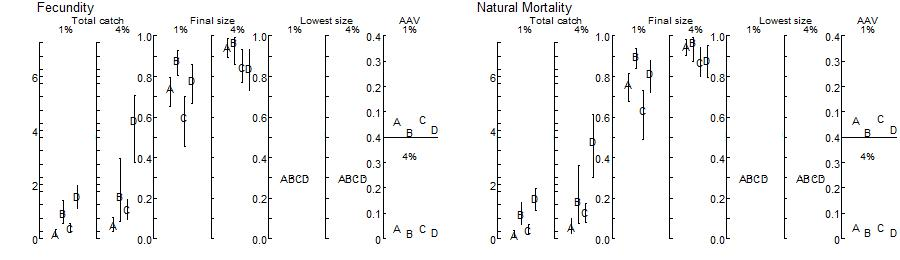
\includegraphics[]{SC66aRMP10_Part2_T1-R.jpeg}
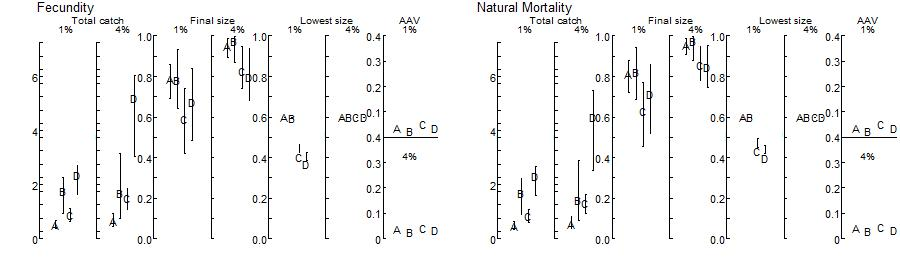
\includegraphics[]{SC66aRMP10_Part2_T1-S.jpeg}
\caption{
Zeh plots for the base-case model
(A = 100-year current, B = 300-year current, C = 100-year alternate, and D = 300-year alternate)
when initial depletion is 30\% (upper panel) and 60\% (lower panel).
Results are shown when density-dependence impacts fecundity (left panel) and when it impacts natural mortality (right panel).
}
\end{figure}



\begin{figure}[H]
\centering
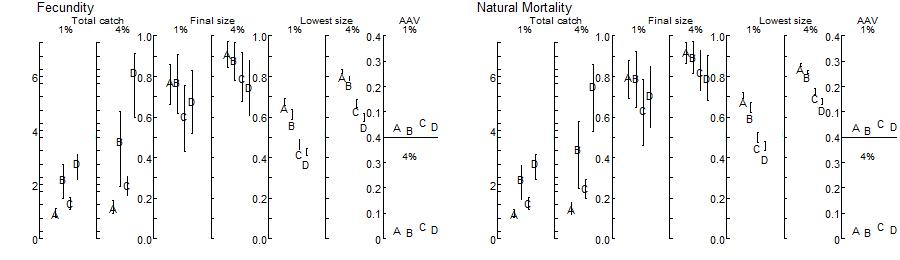
\includegraphics[]{SC66aRMP10_Part2_T1-D.jpeg}
\caption{
Zeh plots for the base-case model
(A = 100-year current, B = 300-year current, C = 100-year alternate, and D = 300-year alternate)
when initial depletion is 99\%.
Results are shown when density-dependence impacts fecundity (left panel) and when it impacts natural mortality (right panel).
}
\end{figure}

\clearpage
%%%%%%%%%%%%%%%%%%%%%%%%%%%%%%%%%%%%%%%%%%%%%%%%%%%%%%%%%%%%%%%%%%%%%%%%%%%%%%%
%%%%%%%%%%%%%%%%%%%%%%%%%%%%%%%%%%%%%%%%%%%%%%%%%%%%%%%%%%%%%%%%%%%%%%%%%%%%%%%
%%%% T4: Initial population P = 0.2
%%%%%%%%%%%%%%%%%%%%%%%%%%%%%%%%%%%%%%%%%%%%%%%%%%%%%%%%%%%%%%%%%%%%%%%%%%%%%%%
%%%%%%%%%%%%%%%%%%%%%%%%%%%%%%%%%%%%%%%%%%%%%%%%%%%%%%%%%%%%%%%%%%%%%%%%%%%%%%%
\phantomsection
\renewcommand{\thefigure}{\thesection}
\stepcounter{section}
\setcounter{figure}{0}


\begin{figure}[H]
\centering
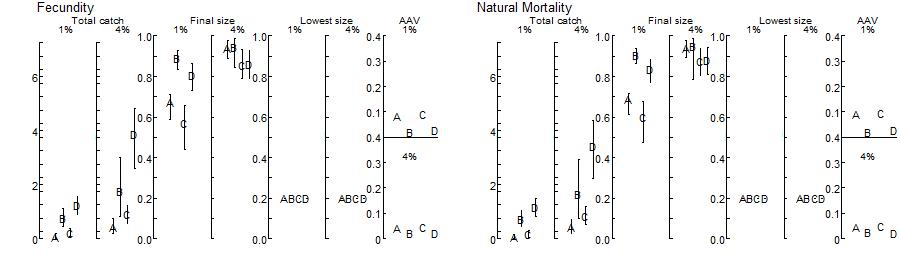
\includegraphics[]{SC66aRMP10_Part2_T1-cC.jpeg}
\caption{
Zeh plots for trial T1-T
[$P_0 $ = 0.2]
(A = 100-year current, B = 300-year current, C = 100-year alternate, and D = 300-year alternate)
when initial depletion is 20\%.
Results are shown when density-dependence impacts fecundity (left panel) and when it impacts natural mortality (right panel).
}
\end{figure}

%%%%%%%%%%%%%%%%%%%%%%%%%%%%%%%%%%%%%%%%%%%%%%%%%%%%%%%%%%%%%%%%%%%%%%%%%%%%%%%
%%%%%%%%%%%%%%%%%%%%%%%%%%%%%%%%%%%%%%%%%%%%%%%%%%%%%%%%%%%%%%%%%%%%%%%%%%%%%%%
%%%% T4: Initial population P = 0.2
%%%%%%%%%%%%%%%%%%%%%%%%%%%%%%%%%%%%%%%%%%%%%%%%%%%%%%%%%%%%%%%%%%%%%%%%%%%%%%%
%%%%%%%%%%%%%%%%%%%%%%%%%%%%%%%%%%%%%%%%%%%%%%%%%%%%%%%%%%%%%%%%%%%%%%%%%%%%%%%
\phantomsection
\stepcounter{section}
\setcounter{figure}{0}


\begin{figure}[H]
\centering
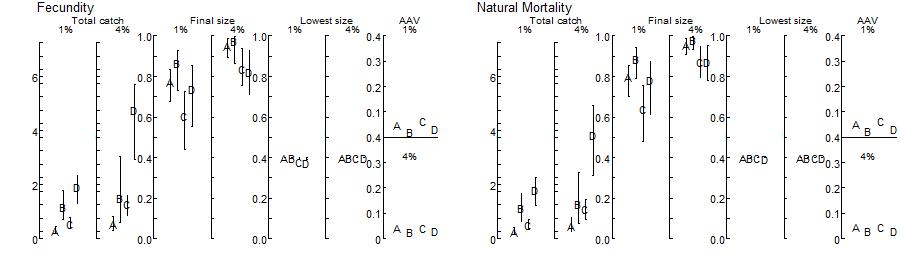
\includegraphics[]{SC66aRMP10_Part2_T1-cD.jpeg}
\caption{
Zeh plots for trial T1-F
[$P_0 $ = 0.4]
(A = 100-year current, B = 300-year current, C = 100-year alternate, and D = 300-year alternate)
when initial depletion is 40\%.
Results are shown when density-dependence impacts fecundity (left panel) and when it impacts natural mortality (right panel).
}
\end{figure}

%%%%%%%%%%%%%%%%%%%%%%%%%%%%%%%%%%%%%%%%%%%%%%%%%%%%%%%%%%%%%%%%%%%%%%%%%%%%%%%
%%%%%%%%%%%%%%%%%%%%%%%%%%%%%%%%%%%%%%%%%%%%%%%%%%%%%%%%%%%%%%%%%%%%%%%%%%%%%%%
%%%% T2: Survey bias 0.5 D,R
%%%%%%%%%%%%%%%%%%%%%%%%%%%%%%%%%%%%%%%%%%%%%%%%%%%%%%%%%%%%%%%%%%%%%%%%%%%%%%%
%%%%%%%%%%%%%%%%%%%%%%%%%%%%%%%%%%%%%%%%%%%%%%%%%%%%%%%%%%%%%%%%%%%%%%%%%%%%%%%
\phantomsection
\stepcounter{section}
\setcounter{figure}{0}


\begin{figure}[H]
\centering
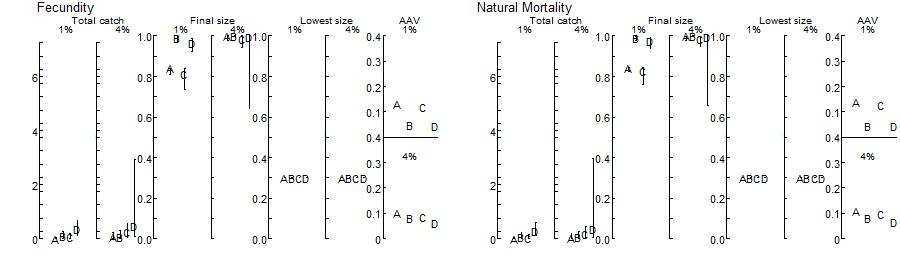
\includegraphics[]{SC66aRMP10_Part2_T2-R.jpeg}
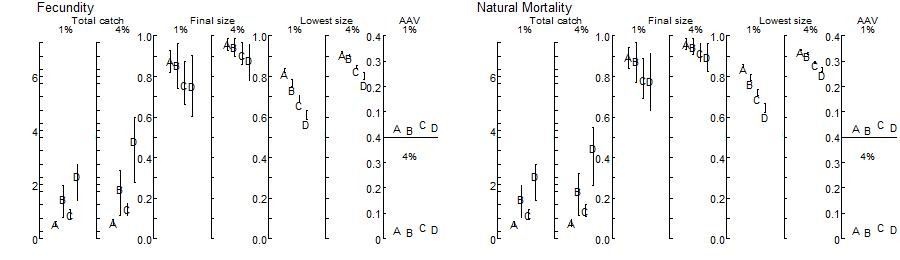
\includegraphics[]{SC66aRMP10_Part2_T2-D.jpeg}
\caption{
Zeh plots for trial T2
[survey bias = 0.5]
(A = 100-year current, B = 300-year current, C = 100-year alternate, and D = 300-year alternate)
when initial depletion is 30\% (upper panel) and 99\% (lower panel).
Results are shown when density-dependence impacts fecundity (left panel) and when it impacts natural mortality (right panel).
}
\end{figure}

%%%%%%%%%%%%%%%%%%%%%%%%%%%%%%%%%%%%%%%%%%%%%%%%%%%%%%%%%%%%%%%%%%%%%%%%%%%%%%%
%%%%%%%%%%%%%%%%%%%%%%%%%%%%%%%%%%%%%%%%%%%%%%%%%%%%%%%%%%%%%%%%%%%%%%%%%%%%%%%
%%%% T3: Survey bias 1.5 D,R,S
%%%%%%%%%%%%%%%%%%%%%%%%%%%%%%%%%%%%%%%%%%%%%%%%%%%%%%%%%%%%%%%%%%%%%%%%%%%%%%%
%%%%%%%%%%%%%%%%%%%%%%%%%%%%%%%%%%%%%%%%%%%%%%%%%%%%%%%%%%%%%%%%%%%%%%%%%%%%%%%
\phantomsection
\renewcommand{\thefigure}{\thesection(\alph{figure})}
\stepcounter{section}
\setcounter{figure}{0}


\begin{figure}[H]
\centering
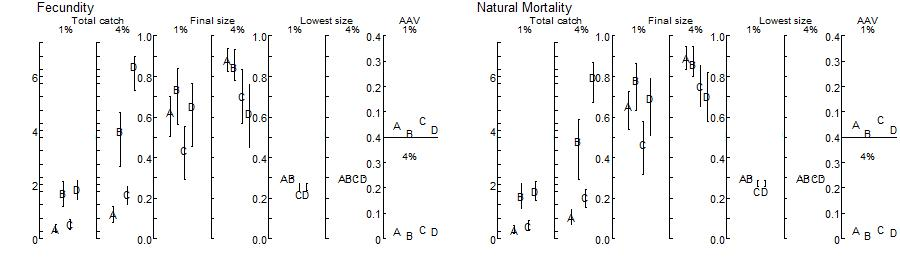
\includegraphics[]{SC66aRMP10_Part2_T3-R.jpeg}
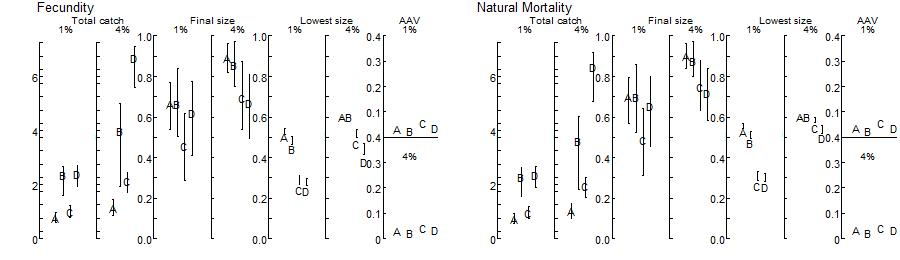
\includegraphics[]{SC66aRMP10_Part2_T3-S.jpeg}
\caption{
Zeh plots for trial T3
[survey bias = 1.5]
(A = 100-year current, B = 300-year current, C = 100-year alternate, and D = 300-year alternate)
when initial depletion is 30\% (upper panel) and 60\% (lower panel).
Results are shown when density-dependence impacts fecundity (left panel) and when it impacts natural mortality (right panel).
}
\end{figure}



\begin{figure}[H]
\centering
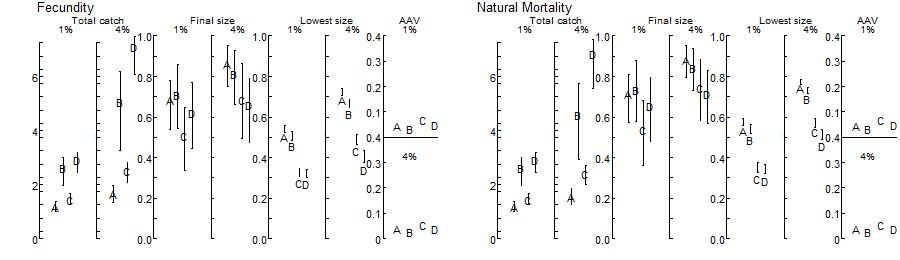
\includegraphics[]{SC66aRMP10_Part2_T3-D.jpeg}
\caption{
Zeh plots for trial T3
[survey bias = 1.5]
(A = 100-year current, B = 300-year current, C = 100-year alternate, and D = 300-year alternate)
when initial depletion is 99\%.
Results are shown when density-dependence impacts fecundity (left panel) and when it impacts natural mortality (right panel).
}
\end{figure}

%%%%%%%%%%%%%%%%%%%%%%%%%%%%%%%%%%%%%%%%%%%%%%%%%%%%%%%%%%%%%%%%%%%%%%%%%%%%%%%
%%%%%%%%%%%%%%%%%%%%%%%%%%%%%%%%%%%%%%%%%%%%%%%%%%%%%%%%%%%%%%%%%%%%%%%%%%%%%%%
%%%% T4: Initial population P = 0.5
%%%%%%%%%%%%%%%%%%%%%%%%%%%%%%%%%%%%%%%%%%%%%%%%%%%%%%%%%%%%%%%%%%%%%%%%%%%%%%%
%%%%%%%%%%%%%%%%%%%%%%%%%%%%%%%%%%%%%%%%%%%%%%%%%%%%%%%%%%%%%%%%%%%%%%%%%%%%%%%
\phantomsection
\renewcommand{\thefigure}{\thesection}
\stepcounter{section}
\setcounter{figure}{0}


\begin{figure}[H]
\centering
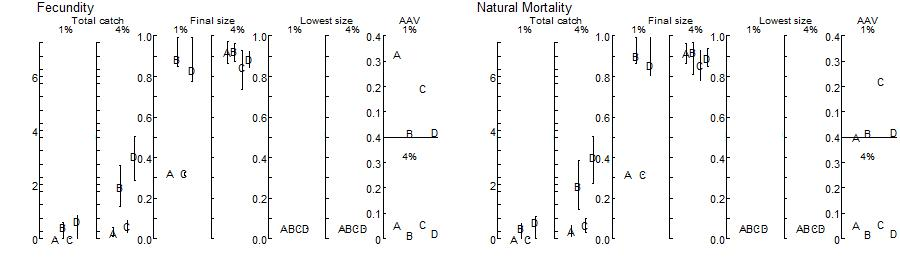
\includegraphics[]{SC66aRMP10_Part2_T4-R.jpeg}
\caption{
Zeh plots for trial T4
[$P_0 $ = 0.05]
(A = 100-year current, B = 300-year current, C = 100-year alternate, and D = 300-year alternate)
when initial depletion is 5\%.
Results are shown when density-dependence impacts fecundity (left panel) and when it impacts natural mortality (right panel).
}
\end{figure}

%%%%%%%%%%%%%%%%%%%%%%%%%%%%%%%%%%%%%%%%%%%%%%%%%%%%%%%%%%%%%%%%%%%%%%%%%%%%%%%
%%%%%%%%%%%%%%%%%%%%%%%%%%%%%%%%%%%%%%%%%%%%%%%%%%%%%%%%%%%%%%%%%%%%%%%%%%%%%%%
%%%% T5: Initial population P = 0.5
%%%%%%%%%%%%%%%%%%%%%%%%%%%%%%%%%%%%%%%%%%%%%%%%%%%%%%%%%%%%%%%%%%%%%%%%%%%%%%%
%%%%%%%%%%%%%%%%%%%%%%%%%%%%%%%%%%%%%%%%%%%%%%%%%%%%%%%%%%%%%%%%%%%%%%%%%%%%%%%
\phantomsection
\stepcounter{section}
\setcounter{figure}{0}


\begin{figure}[H]
\centering
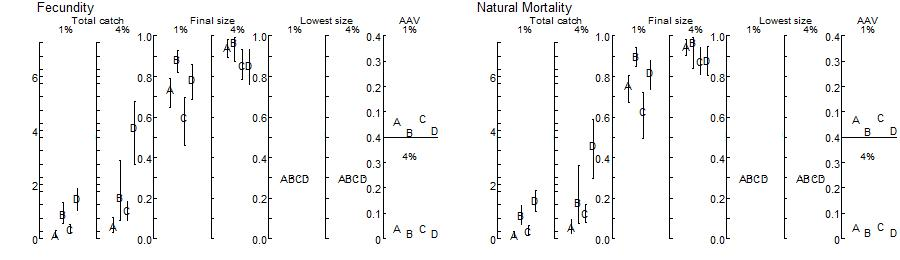
\includegraphics[]{SC66aRMP10_Part2_T5-R.jpeg}
\caption{
Zeh plots for trial T5
[years of protection = 25]
(A = 100-year current, B = 300-year current, C = 100-year alternate, and D = 300-year alternate)
when initial depletion is 30\%.
Results are shown when density-dependence impacts fecundity (left panel) and when it impacts natural mortality (right panel).
}
\end{figure}

%%%%%%%%%%%%%%%%%%%%%%%%%%%%%%%%%%%%%%%%%%%%%%%%%%%%%%%%%%%%%%%%%%%%%%%%%%%%%%%
%%%%%%%%%%%%%%%%%%%%%%%%%%%%%%%%%%%%%%%%%%%%%%%%%%%%%%%%%%%%%%%%%%%%%%%%%%%%%%%
%%%% T6: Initial population P = 0.5
%%%%%%%%%%%%%%%%%%%%%%%%%%%%%%%%%%%%%%%%%%%%%%%%%%%%%%%%%%%%%%%%%%%%%%%%%%%%%%%
%%%%%%%%%%%%%%%%%%%%%%%%%%%%%%%%%%%%%%%%%%%%%%%%%%%%%%%%%%%%%%%%%%%%%%%%%%%%%%%
\phantomsection
\stepcounter{section}
\setcounter{figure}{0}


\begin{figure}[H]
\centering
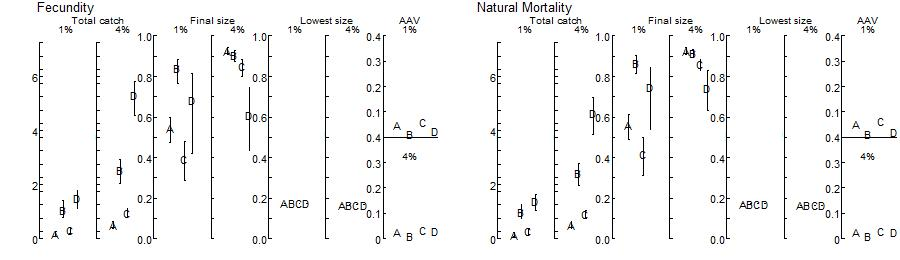
\includegraphics[]{SC66aRMP10_Part2_T6-R.jpeg}
\caption{
Zeh plots for trial T6
[1/2 true catch]
(A = 100-year current, B = 300-year current, C = 100-year alternate, and D = 300-year alternate)
when initial depletion is 30\%.
Results are shown when density-dependence impacts fecundity (left panel) and when it impacts natural mortality (right panel).
}
\end{figure}

%%%%%%%%%%%%%%%%%%%%%%%%%%%%%%%%%%%%%%%%%%%%%%%%%%%%%%%%%%%%%%%%%%%%%%%%%%%%%%%
%%%%%%%%%%%%%%%%%%%%%%%%%%%%%%%%%%%%%%%%%%%%%%%%%%%%%%%%%%%%%%%%%%%%%%%%%%%%%%%
%%%% T7: Age at maturity 7 years
%%%%%%%%%%%%%%%%%%%%%%%%%%%%%%%%%%%%%%%%%%%%%%%%%%%%%%%%%%%%%%%%%%%%%%%%%%%%%%%
%%%%%%%%%%%%%%%%%%%%%%%%%%%%%%%%%%%%%%%%%%%%%%%%%%%%%%%%%%%%%%%%%%%%%%%%%%%%%%%
\phantomsection
\stepcounter{section}
\setcounter{figure}{0}


\begin{figure}[H]
\centering
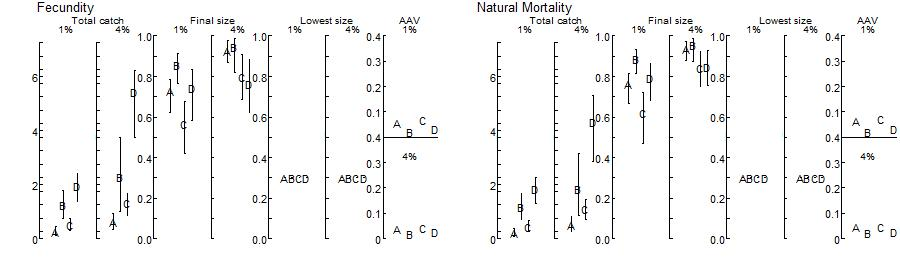
\includegraphics[]{SC66aRMP10_Part2_T7-R.jpeg}
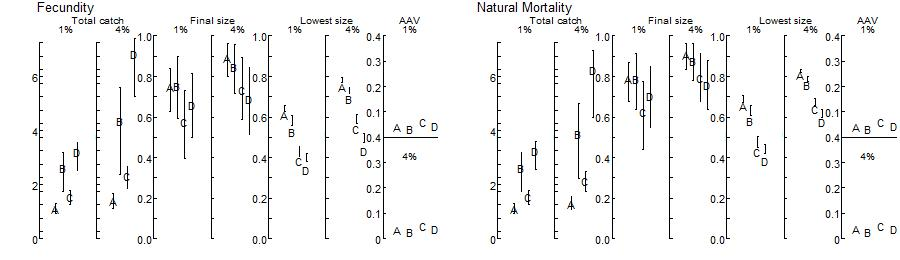
\includegraphics[]{SC66aRMP10_Part2_T7-D.jpeg}
\caption{
Zeh plots for trial T7
[age at maturity = 10]
(A = 100-year current, B = 300-year current, C = 100-year alternate, and D = 300-year alternate)
when initial depletion is 30\% (upper panel) and 99\% (lower panel).
Results are shown when density-dependence impacts fecundity (left panel) and when it impacts natural mortality (right panel).
}
\end{figure}

%%%%%%%%%%%%%%%%%%%%%%%%%%%%%%%%%%%%%%%%%%%%%%%%%%%%%%%%%%%%%%%%%%%%%%%%%%%%%%%
%%%%%%%%%%%%%%%%%%%%%%%%%%%%%%%%%%%%%%%%%%%%%%%%%%%%%%%%%%%%%%%%%%%%%%%%%%%%%%%
%%%% T8: Random parameters not done
%%%%%%%%%%%%%%%%%%%%%%%%%%%%%%%%%%%%%%%%%%%%%%%%%%%%%%%%%%%%%%%%%%%%%%%%%%%%%%%
%%%%%%%%%%%%%%%%%%%%%%%%%%%%%%%%%%%%%%%%%%%%%%%%%%%%%%%%%%%%%%%%%%%%%%%%%%%%%%%

%%%%%%%%%%%%%%%%%%%%%%%%%%%%%%%%%%%%%%%%%%%%%%%%%%%%%%%%%%%%%%%%%%%%%%%%%%%%%%%
%%%%%%%%%%%%%%%%%%%%%%%%%%%%%%%%%%%%%%%%%%%%%%%%%%%%%%%%%%%%%%%%%%%%%%%%%%%%%%%
%%%% T9: Episodic events (Not currently implemented)
%%%%%%%%%%%%%%%%%%%%%%%%%%%%%%%%%%%%%%%%%%%%%%%%%%%%%%%%%%%%%%%%%%%%%%%%%%%%%%%
%%%%%%%%%%%%%%%%%%%%%%%%%%%%%%%%%%%%%%%%%%%%%%%%%%%%%%%%%%%%%%%%%%%%%%%%%%%%%%%
% \phantomsection
% \stepcounter{section}
% \setcounter{figure}{0}
% <<echo = FALSE, include = FALSE>>=
% keep <- subset(sheet, depl %in% c(0.3) & T == "T9")
% if (NROW(keep) > 4) stop("Too many factors selected")
% plotnamea <- as.character(keep$name)[1]
% plotnamea <- paste(paper, substring(plotnamea, 4, nchar(plotnamea) - 1), sep = "_")
% depl <- formatC(keep$depl * 100, format = "f", digits = 0)[1]
% plot_curve(aep100, aep300, ps4100, ps4300, keep, plotnamea, part = 2)

% keep <- subset(sheet, depl %in% c(0.99) & T == "T9")
% if (NROW(keep) > 4) stop("Too many factors selected")
% plotnameb <- as.character(keep$name)[1]
% plotnameb <- paste(paper, substring(plotnameb, 4, nchar(plotnameb) - 1), sep = "_")
% depl[2] <- formatC(keep$depl * 100, format = "f", digits = 0)[1]
% plot_curve(aep100, aep300, ps4100, ps4300, keep, plotnameb, part = 2)
% @

% \begin{figure}[H]
% \centering
% \includegraphics[]{paste(plotnamea, "jpeg", sep = ".")}
% \includegraphics[]{paste(plotnameb, "jpeg", sep = ".")}
% \caption{
% Zeh plots for trial as.character(keep$T[1])
% [Episodic events]
% (A = 100-year current, B = 300-year current, C = 100-year alternate, and D = 300-year alternate)
% when initial depletion is depl[1]\% (upper panel) and depl[2]\% (lower panel).
% Results are shown when density-dependence impacts fecundity (left panel) and when it impacts natural mortality (right panel).
% }
% \end{figure}

%%%%%%%%%%%%%%%%%%%%%%%%%%%%%%%%%%%%%%%%%%%%%%%%%%%%%%%%%%%%%%%%%%%%%%%%%%%%%%%
%%%%%%%%%%%%%%%%%%%%%%%%%%%%%%%%%%%%%%%%%%%%%%%%%%%%%%%%%%%%%%%%%%%%%%%%%%%%%%%
%%%% T10: MSYL = 0.04 bad
%%%%%%%%%%%%%%%%%%%%%%%%%%%%%%%%%%%%%%%%%%%%%%%%%%%%%%%%%%%%%%%%%%%%%%%%%%%%%%%
%%%%%%%%%%%%%%%%%%%%%%%%%%%%%%%%%%%%%%%%%%%%%%%%%%%%%%%%%%%%%%%%%%%%%%%%%%%%%%%
% \phantomsection
% \stepcounter{section}
% \setcounter{figure}{0}
% <<echo = FALSE, include = FALSE>>=
% keep <- subset(sheet, depl %in% c(0.3) & T == "T10A")
% if (NROW(keep) > 4) stop("Too many factors selected")
% plotnamea <- as.character(keep$name)[1]
% plotnamea <- paste(paper, substring(plotnamea, 4, nchar(plotnamea) - 1), sep = "_")
% depl <- formatC(keep$depl * 100, format = "f", digits = 0)[1]
% plot_curve(aep100, aep300, ps4100, ps4300, keep, plotnamea, part = 2)

% keep <- subset(sheet, depl %in% c(0.99) & T == "T10A")
% if (NROW(keep) > 4) stop("Too many factors selected")
% plotnameb <- as.character(keep$name)[1]
% plotnameb <- paste(paper, substring(plotnameb, 4, nchar(plotnameb) - 1), sep = "_")
% depl[2] <- formatC(keep$depl * 100, format = "f", digits = 0)[1]
% plot_curve(aep100, aep300, ps4100, ps4300, keep, plotnameb, part = 2)
% @

% \begin{figure}[H]
% \centering
% \includegraphics[]{paste(plotnamea, "jpeg", sep = ".")}
% \includegraphics[]{paste(plotnameb, "jpeg", sep = ".")}
% \caption{
% Zeh plots for trial as.character(keep$T[1])
% [MSYL = keep$msyl[1] * 100\%]
% (A = 100-year current, B = 300-year current, C = 100-year alternate, and D = 300-year alternate)
% when initial depletion is depl[1]\% (upper panel) and depl[2]\% (lower panel).
% Results are shown when density-dependence impacts fecundity (left panel) and when it impacts natural mortality (right panel).
% }
% \end{figure}

%%%%%%%%%%%%%%%%%%%%%%%%%%%%%%%%%%%%%%%%%%%%%%%%%%%%%%%%%%%%%%%%%%%%%%%%%%%%%%%
%%%%%%%%%%%%%%%%%%%%%%%%%%%%%%%%%%%%%%%%%%%%%%%%%%%%%%%%%%%%%%%%%%%%%%%%%%%%%%%
%%%% T11: MSYL = 0.08
%%%%%%%%%%%%%%%%%%%%%%%%%%%%%%%%%%%%%%%%%%%%%%%%%%%%%%%%%%%%%%%%%%%%%%%%%%%%%%%
%%%%%%%%%%%%%%%%%%%%%%%%%%%%%%%%%%%%%%%%%%%%%%%%%%%%%%%%%%%%%%%%%%%%%%%%%%%%%%%
\phantomsection
\stepcounter{section}
\setcounter{figure}{0}


\begin{figure}[H]
\centering
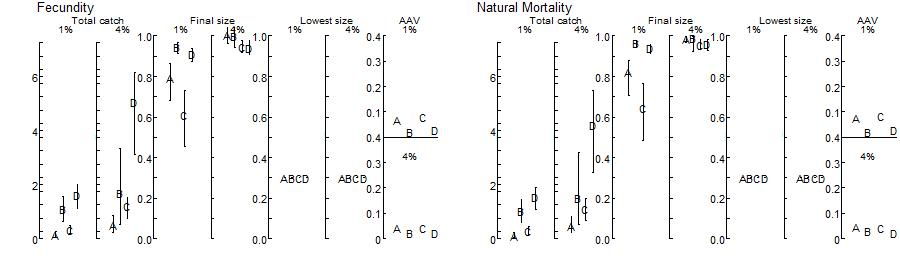
\includegraphics[]{SC66aRMP10_Part2_T11A-R.jpeg}
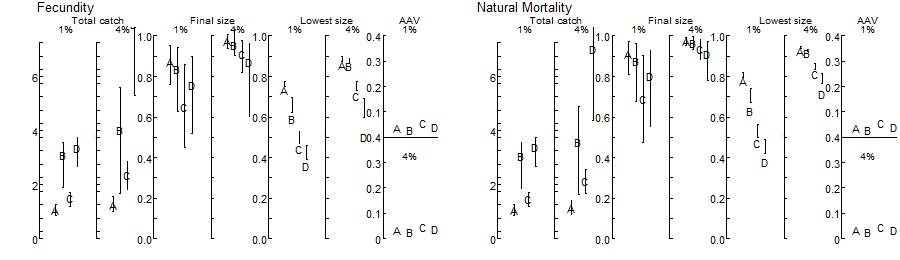
\includegraphics[]{SC66aRMP10_Part2_T11A-D.jpeg}
\caption{
Zeh plots for trial T11A
[MSYL = 80\%]
(A = 100-year current, B = 300-year current, C = 100-year alternate, and D = 300-year alternate)
when initial depletion is 30\% (upper panel) and 99\% (lower panel).
Results are shown when density-dependence impacts fecundity (left panel) and when it impacts natural mortality (right panel).
}
\end{figure}

%%%%%%%%%%%%%%%%%%%%%%%%%%%%%%%%%%%%%%%%%%%%%%%%%%%%%%%%%%%%%%%%%%%%%%%%%%%%%%%
%%%%%%%%%%%%%%%%%%%%%%%%%%%%%%%%%%%%%%%%%%%%%%%%%%%%%%%%%%%%%%%%%%%%%%%%%%%%%%%
%%%% T12A: 2*K over management period
%%%%%%%%%%%%%%%%%%%%%%%%%%%%%%%%%%%%%%%%%%%%%%%%%%%%%%%%%%%%%%%%%%%%%%%%%%%%%%%
%%%%%%%%%%%%%%%%%%%%%%%%%%%%%%%%%%%%%%%%%%%%%%%%%%%%%%%%%%%%%%%%%%%%%%%%%%%%%%%
\phantomsection
\stepcounter{section}
\setcounter{figure}{0}


\begin{figure}[H]
\centering
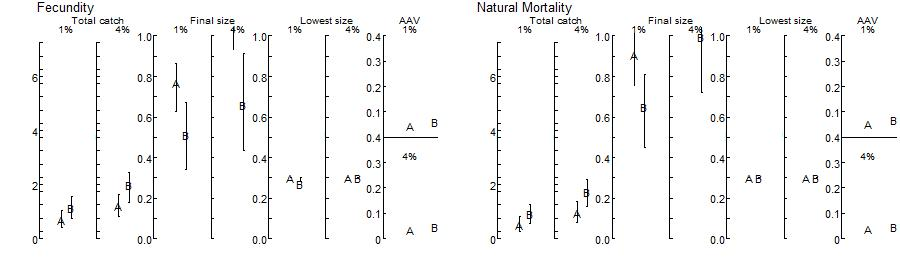
\includegraphics[]{SC66aRMP10_Part2_T12A-R.jpeg}
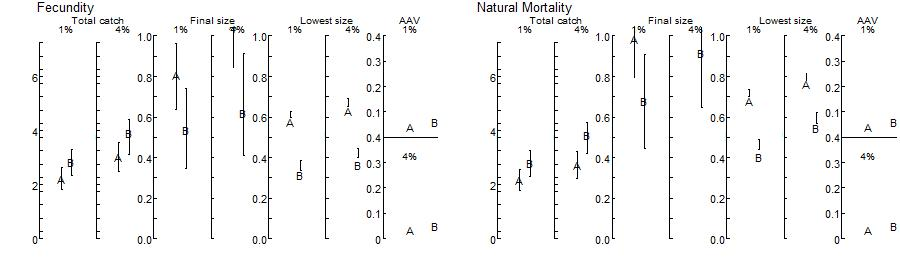
\includegraphics[]{SC66aRMP10_Part2_T12A-D.jpeg}
\caption{
Zeh plots for trial T12A
[linear change to 2$K$ over management period]
(A = 100-year current and B = 100-year alternate)
when initial depletion is 30\% (upper panel) and 99\% (lower panel).
Results are shown when density-dependence impacts fecundity (left panel) and when it impacts natural mortality (right panel).
}
\end{figure}

%%%%%%%%%%%%%%%%%%%%%%%%%%%%%%%%%%%%%%%%%%%%%%%%%%%%%%%%%%%%%%%%%%%%%%%%%%%%%%%
%%%%%%%%%%%%%%%%%%%%%%%%%%%%%%%%%%%%%%%%%%%%%%%%%%%%%%%%%%%%%%%%%%%%%%%%%%%%%%%
%%%% T12B: 0.5*K over management period
%%%%%%%%%%%%%%%%%%%%%%%%%%%%%%%%%%%%%%%%%%%%%%%%%%%%%%%%%%%%%%%%%%%%%%%%%%%%%%%
%%%%%%%%%%%%%%%%%%%%%%%%%%%%%%%%%%%%%%%%%%%%%%%%%%%%%%%%%%%%%%%%%%%%%%%%%%%%%%%
\phantomsection
\stepcounter{section}
\setcounter{figure}{0}


\begin{figure}[H]
\centering
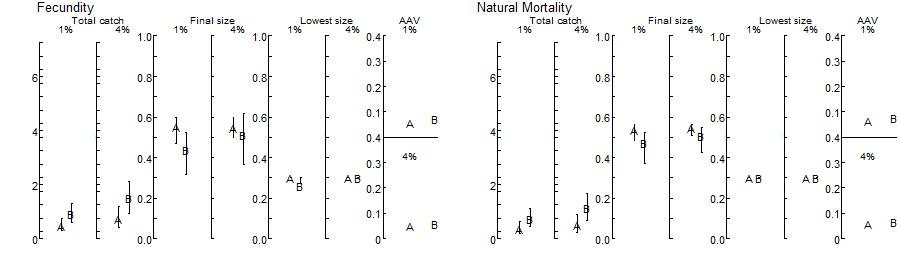
\includegraphics[]{SC66aRMP10_Part2_T12B-R.jpeg}
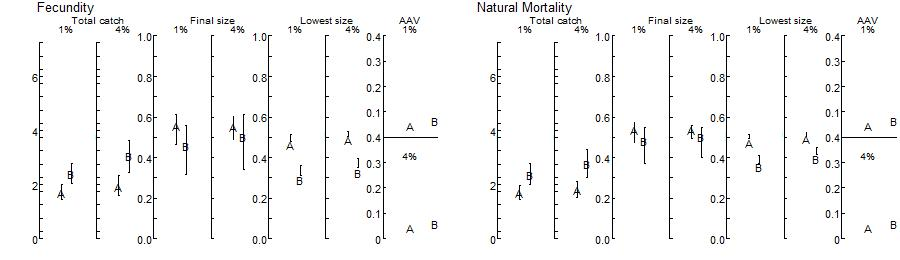
\includegraphics[]{SC66aRMP10_Part2_T12B-D.jpeg}
\caption{
Zeh plots for trial T12B
[linear change to 0.5$K$ over management period]
(A = 100-year current and B = 100-year alternate)
when initial depletion is 30\% (upper panel) and 99\% (lower panel).
Results are shown when density-dependence impacts fecundity (left panel) and when it impacts natural mortality (right panel).
}
\end{figure}

%%%%%%%%%%%%%%%%%%%%%%%%%%%%%%%%%%%%%%%%%%%%%%%%%%%%%%%%%%%%%%%%%%%%%%%%%%%%%%%
%%%%%%%%%%%%%%%%%%%%%%%%%%%%%%%%%%%%%%%%%%%%%%%%%%%%%%%%%%%%%%%%%%%%%%%%%%%%%%%
%%%% T13: 33 yr 141
%%%%%%%%%%%%%%%%%%%%%%%%%%%%%%%%%%%%%%%%%%%%%%%%%%%%%%%%%%%%%%%%%%%%%%%%%%%%%%%
%%%%%%%%%%%%%%%%%%%%%%%%%%%%%%%%%%%%%%%%%%%%%%%%%%%%%%%%%%%%%%%%%%%%%%%%%%%%%%%
\phantomsection
\stepcounter{section}
\setcounter{figure}{0}


\begin{figure}[H]
\centering
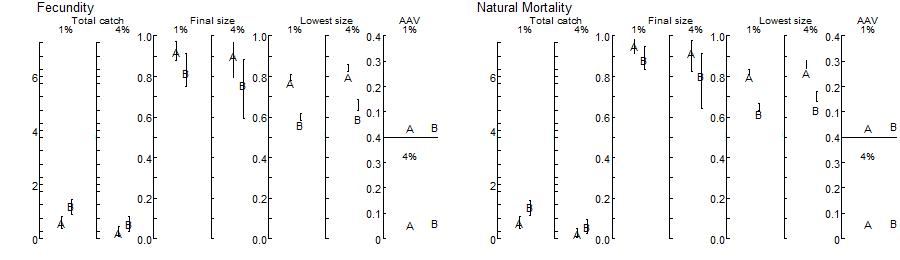
\includegraphics[]{SC66aRMP10_Part2_T13B-R.jpeg}
% \includegraphics[]{paste(plotnameb, "jpeg", sep = ".")}
\caption{
Zeh plots for trial 13
[33 year cycle in $MSYR$ (141) and (414)]
(A = 100-year current, B = 300-year current, C = 100-year alternate, and D = 300-year alternate)
when initial depletion is 30\% .% (upper panel) and NA\% (lower panel).
Results are shown when density-dependence impacts fecundity (left panel) and when it impacts natural mortality (right panel).
}
\end{figure}

% %%%%%%%%%%%%%%%%%%%%%%%%%%%%%%%%%%%%%%%%%%%%%%%%%%%%%%%%%%%%%%%%%%%%%%%%%%%%%%%
% %%%%%%%%%%%%%%%%%%%%%%%%%%%%%%%%%%%%%%%%%%%%%%%%%%%%%%%%%%%%%%%%%%%%%%%%%%%%%%%
% %%%% T13: 33 yr 141
% %%%%%%%%%%%%%%%%%%%%%%%%%%%%%%%%%%%%%%%%%%%%%%%%%%%%%%%%%%%%%%%%%%%%%%%%%%%%%%%
% %%%%%%%%%%%%%%%%%%%%%%%%%%%%%%%%%%%%%%%%%%%%%%%%%%%%%%%%%%%%%%%%%%%%%%%%%%%%%%%
% \phantomsection
% \stepcounter{section}
% \setcounter{figure}{0}
% <<echo = FALSE, include = FALSE>>=
% keep <- subset(sheet, depl %in% c(0.3) & T == "T13A")
% if (NROW(keep) > 4) stop("Too many factors selected")
% plotnamea <- as.character(keep$name)[1]
% plotnamea <- paste(paper, substring(plotnamea, 4, nchar(plotnamea) - 1), sep = "_")
% depl <- formatC(keep$depl * 100, format = "f", digits = 0)[1]
% plot_curve(aep100, aep300, ps4100, ps4300, keep, plotnamea, part = 2)

% keep <- subset(sheet, depl %in% c(0.99) & T == "T13A")
% if (NROW(keep) > 4) stop("Too many factors selected")
% plotnameb <- as.character(keep$name)[1]
% plotnameb <- paste(paper, substring(plotnameb, 4, nchar(plotnameb) - 1), sep = "_")
% depl[2] <- formatC(keep$depl * 100, format = "f", digits = 0)[1]
% plot_curve(aep100, aep300, ps4100, ps4300, keep, plotnameb, part = 2)
% @

% \begin{figure}[H]
% \centering
% \includegraphics[]{paste(plotnamea, "jpeg", sep = ".")}
% \includegraphics[]{paste(plotnameb, "jpeg", sep = ".")}
% \caption{
% Zeh plots for trial 13
% [keep$istep[1] year cycle in $MSYR$ (414)]
% (A = 100-year current and B = 100-year alternate)
% when initial depletion is depl[1]\% (upper panel) and depl[2]\% (lower panel).
% Results are shown when density-dependence impacts fecundity (left panel) and when it impacts natural mortality (right panel).
% }
% \end{figure}

%%%%%%%%%%%%%%%%%%%%%%%%%%%%%%%%%%%%%%%%%%%%%%%%%%%%%%%%%%%%%%%%%%%%%%%%%%%%%%%
%%%%%%%%%%%%%%%%%%%%%%%%%%%%%%%%%%%%%%%%%%%%%%%%%%%%%%%%%%%%%%%%%%%%%%%%%%%%%%%
%%%% T14B: Survey every 10 years
%%%%%%%%%%%%%%%%%%%%%%%%%%%%%%%%%%%%%%%%%%%%%%%%%%%%%%%%%%%%%%%%%%%%%%%%%%%%%%%
%%%%%%%%%%%%%%%%%%%%%%%%%%%%%%%%%%%%%%%%%%%%%%%%%%%%%%%%%%%%%%%%%%%%%%%%%%%%%%%
\phantomsection
\stepcounter{section}
\setcounter{figure}{0}


\begin{figure}[H]
\centering
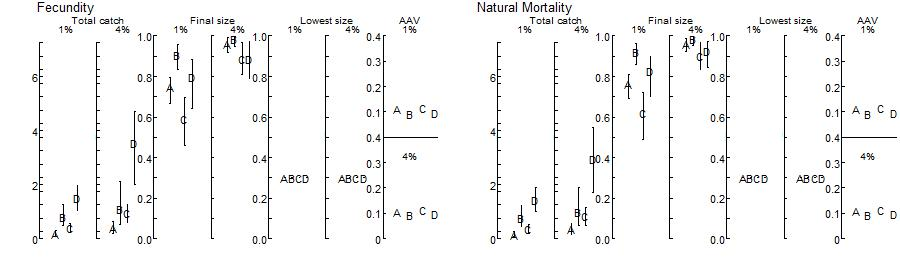
\includegraphics[]{SC66aRMP10_Part2_T14B-R.jpeg}
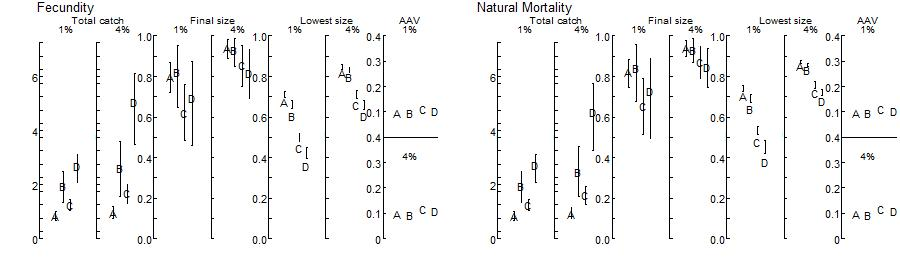
\includegraphics[]{SC66aRMP10_Part2_T14B-D.jpeg}
\caption{
Zeh plots for trial 15
[survey every 10 years]
(A = 100-year current, B = 300-year current, C = 100-year alternate, and D = 300-year alternate)
when initial depletion is 30\% (upper panel) and 99\% (lower panel).
Results are shown when density-dependence impacts fecundity (left panel) and when it impacts natural mortality (right panel).
}
\end{figure}

%%%%%%%%%%%%%%%%%%%%%%%%%%%%%%%%%%%%%%%%%%%%%%%%%%%%%%%%%%%%%%%%%%%%%%%%%%%%%%%
%%%%%%%%%%%%%%%%%%%%%%%%%%%%%%%%%%%%%%%%%%%%%%%%%%%%%%%%%%%%%%%%%%%%%%%%%%%%%%%
%%%% T16: Linear decline in MSYR
%%%%%%%%%%%%%%%%%%%%%%%%%%%%%%%%%%%%%%%%%%%%%%%%%%%%%%%%%%%%%%%%%%%%%%%%%%%%%%%
%%%%%%%%%%%%%%%%%%%%%%%%%%%%%%%%%%%%%%%%%%%%%%%%%%%%%%%%%%%%%%%%%%%%%%%%%%%%%%%
\phantomsection
\stepcounter{section}
\setcounter{figure}{0}


\begin{figure}[H]
\centering
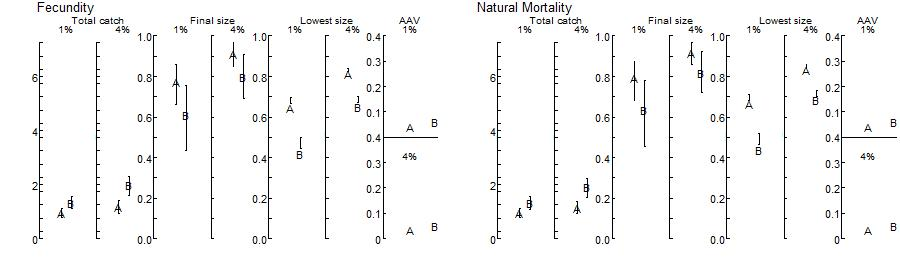
\includegraphics[]{SC66aRMP10_Part2_T17-D.jpeg}
\caption{
Zeh plots for trial 16
[linear change to 0.5$MSYR$]
(A = 100-year current and B = 100-year alternate)
when initial depletion is 99\%.
Results are shown when density-dependence impacts fecundity (left panel) and when it impacts natural mortality (right panel).
}
\end{figure}

%%%%%%%%%%%%%%%%%%%%%%%%%%%%%%%%%%%%%%%%%%%%%%%%%%%%%%%%%%%%%%%%%%%%%%%%%%%%%%%
%%%%%%%%%%%%%%%%%%%%%%%%%%%%%%%%%%%%%%%%%%%%%%%%%%%%%%%%%%%%%%%%%%%%%%%%%%%%%%%
%%%% T17: Linear decline in MSYR and K
%%%%%%%%%%%%%%%%%%%%%%%%%%%%%%%%%%%%%%%%%%%%%%%%%%%%%%%%%%%%%%%%%%%%%%%%%%%%%%%
%%%%%%%%%%%%%%%%%%%%%%%%%%%%%%%%%%%%%%%%%%%%%%%%%%%%%%%%%%%%%%%%%%%%%%%%%%%%%%%
\phantomsection
\stepcounter{section}
\setcounter{figure}{0}


\begin{figure}[H]
\centering
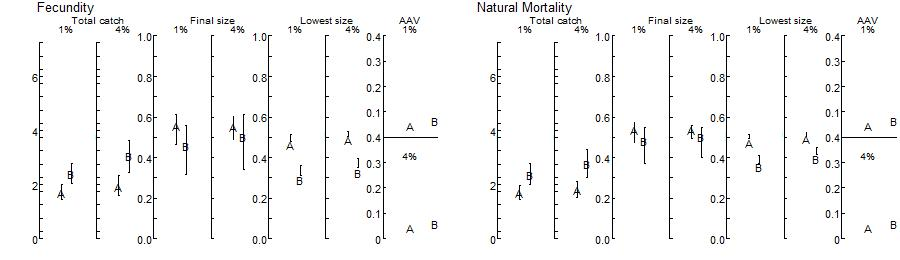
\includegraphics[]{SC66aRMP10_Part2_T19-D.jpeg}
\caption{
Zeh plots for trial 17
[linear change to 0.5$MSYR$ and 0.5$K$]
(A = 100-year current and B = 100-year alternate)
when initial depletion is 99\%.
Results are shown when density-dependence impacts fecundity (left panel) and when it impacts natural mortality (right panel).
}
\end{figure}

\clearpage
%%%%%%%%%%%%%%%%%%%%%%%%%%%%%%%%%%%%%%%%%%%%%%%%%%%%%%%%%%%%%%%%%%%%%%%%%%%%%%%
%%%%%%%%%%%%%%%%%%%%%%%%%%%%%%%%%%%%%%%%%%%%%%%%%%%%%%%%%%%%%%%%%%%%%%%%%%%%%%%
%%%% T18: Survey bias 1.5 D,R,S
%%%%%%%%%%%%%%%%%%%%%%%%%%%%%%%%%%%%%%%%%%%%%%%%%%%%%%%%%%%%%%%%%%%%%%%%%%%%%%%
%%%%%%%%%%%%%%%%%%%%%%%%%%%%%%%%%%%%%%%%%%%%%%%%%%%%%%%%%%%%%%%%%%%%%%%%%%%%%%%
\phantomsection
\renewcommand{\thefigure}{\thesection(\alph{figure})}
\stepcounter{section}
\setcounter{figure}{0}


\begin{figure}[H]
\centering
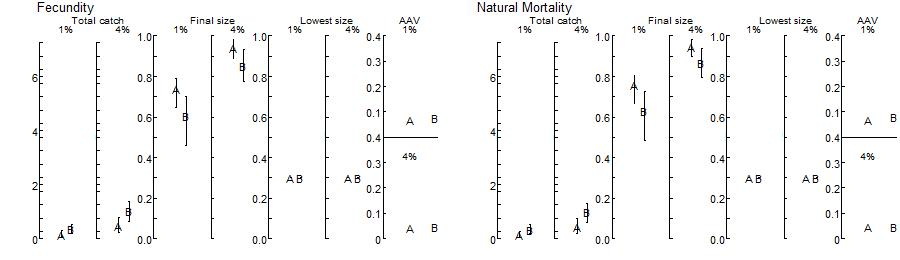
\includegraphics[]{SC66aRMP10_Part2_T18-R.jpeg}
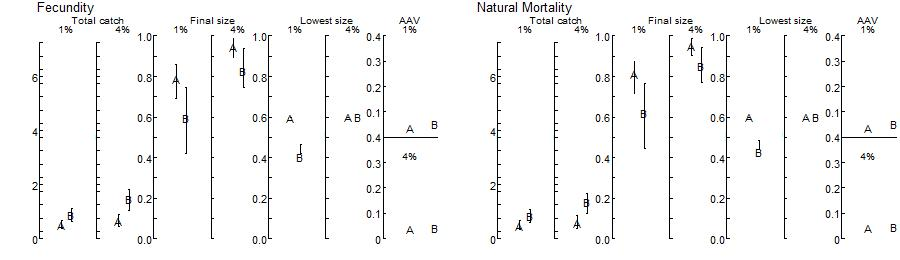
\includegraphics[]{SC66aRMP10_Part2_T18-S.jpeg}
\caption{
Zeh plots for trial T18
[linear change to 2$MSYR$]
(A = 100-year current and B = 100-year alternate)
when initial depletion is 30\% (upper panel) and 60\% (lower panel).
Results are shown when density-dependence impacts fecundity (left panel) and when it impacts natural mortality (right panel).
}
\end{figure}



\begin{figure}[H]
\centering
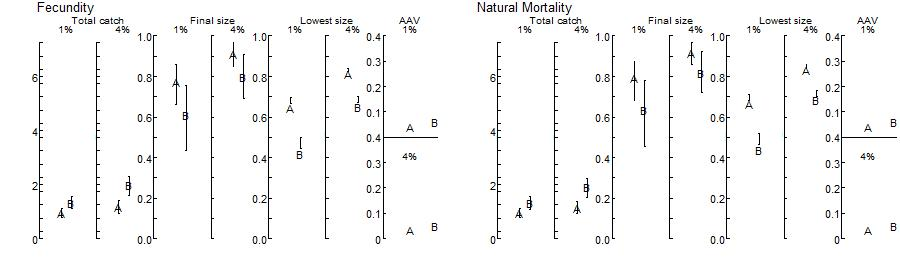
\includegraphics[]{SC66aRMP10_Part2_T18-D.jpeg}
\caption{
Zeh plots for trial T18
[linear change to 2$MSYR$]
(A = 100-year current and B = 100-year alternate)
when initial depletion is 99\%.
Results are shown when density-dependence impacts fecundity (left panel) and when it impacts natural mortality (right panel).
}
\end{figure}

\clearpage
%%%%%%%%%%%%%%%%%%%%%%%%%%%%%%%%%%%%%%%%%%%%%%%%%%%%%%%%%%%%%%%%%%%%%%%%%%%%%%%
%%%%%%%%%%%%%%%%%%%%%%%%%%%%%%%%%%%%%%%%%%%%%%%%%%%%%%%%%%%%%%%%%%%%%%%%%%%%%%%
%%%% T19: Linear decline to 0.5MSYR and 0.5K, with all D,R,S
%%%%%%%%%%%%%%%%%%%%%%%%%%%%%%%%%%%%%%%%%%%%%%%%%%%%%%%%%%%%%%%%%%%%%%%%%%%%%%%
%%%%%%%%%%%%%%%%%%%%%%%%%%%%%%%%%%%%%%%%%%%%%%%%%%%%%%%%%%%%%%%%%%%%%%%%%%%%%%%
\phantomsection
\stepcounter{section}
\setcounter{figure}{0}


\begin{figure}[H]
\centering
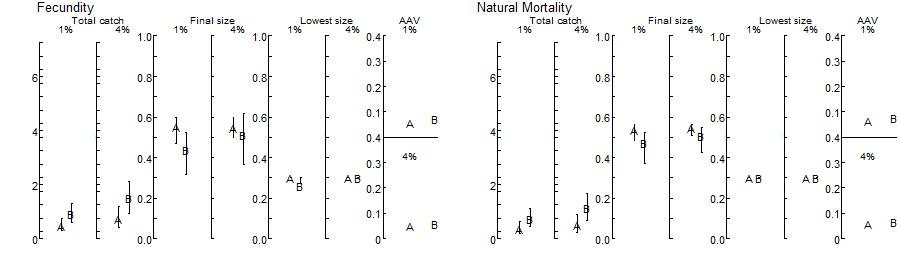
\includegraphics[]{SC66aRMP10_Part2_T19-R.jpeg}
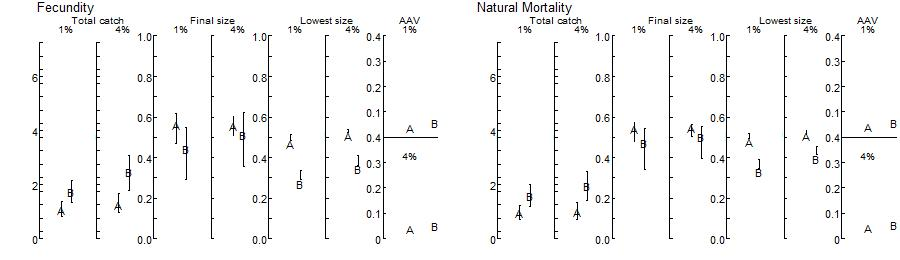
\includegraphics[]{SC66aRMP10_Part2_T19-S.jpeg}
\caption{
Zeh plots for trial T19
[linear change to 0.5$MSYR$ and 0.5$K$]
(A = 100-year current and B = 100-year alternate)
when initial depletion is 30\% (upper panel) and 60\% (lower panel).
Results are shown when density-dependence impacts fecundity (left panel) and when it impacts natural mortality (right panel).
}
\end{figure}



\begin{figure}[H]
\centering
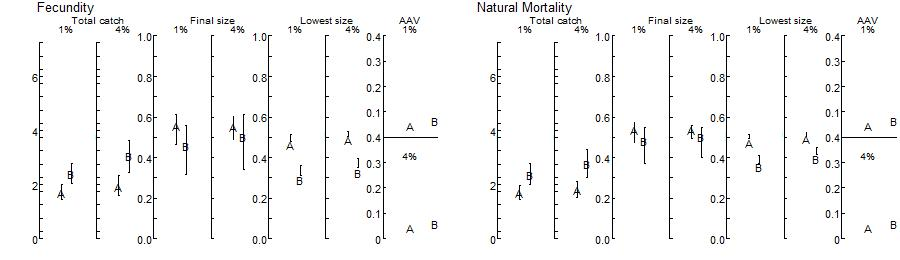
\includegraphics[]{SC66aRMP10_Part2_T19-D.jpeg}
\caption{
Zeh plots for trial T19
[linear change to 0.5$MSYR$ and 0.5$K$]
(A = 100-year current and B = 100-year alternate)
when initial depletion is 99\%.
Results are shown when density-dependence impacts fecundity (left panel) and when it impacts natural mortality (right panel).
}
\end{figure}

\clearpage
%%%%%%%%%%%%%%%%%%%%%%%%%%%%%%%%%%%%%%%%%%%%%%%%%%%%%%%%%%%%%%%%%%%%%%%%%%%%%%%
%%%%%%%%%%%%%%%%%%%%%%%%%%%%%%%%%%%%%%%%%%%%%%%%%%%%%%%%%%%%%%%%%%%%%%%%%%%%%%%
%%%% T20: Episodic events and survey bias 1.5 D,R,S
%%%%%%%%%%%%%%%%%%%%%%%%%%%%%%%%%%%%%%%%%%%%%%%%%%%%%%%%%%%%%%%%%%%%%%%%%%%%%%%
%%%%%%%%%%%%%%%%%%%%%%%%%%%%%%%%%%%%%%%%%%%%%%%%%%%%%%%%%%%%%%%%%%%%%%%%%%%%%%%
\phantomsection
\stepcounter{section}
\setcounter{figure}{0}


\begin{figure}[H]
\centering
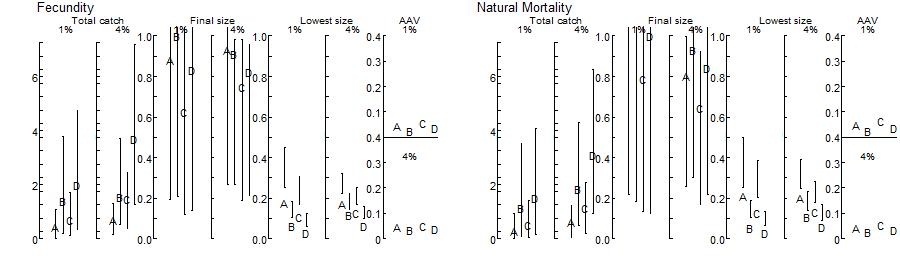
\includegraphics[]{SC66aRMP10_Part2_T20-R.jpeg}
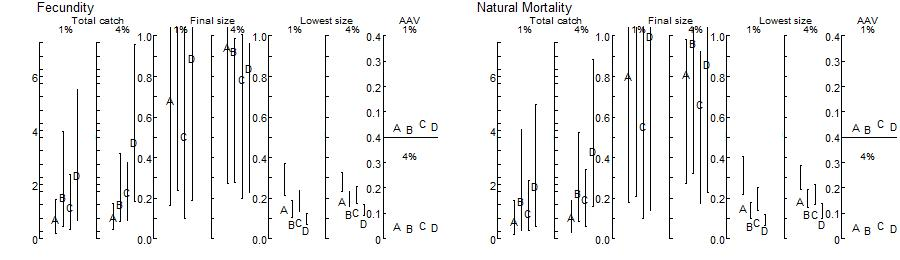
\includegraphics[]{SC66aRMP10_Part2_T20-S.jpeg}
\caption{
Zeh plots for trial T20
[Episodic events and survey bias = 1.5]
(A = 100-year current, B = 300-year current, C = 100-year alternate, and D = 300-year alternate)
when initial depletion is 30\% (upper panel) and 60\% (lower panel).
Results are shown when density-dependence impacts fecundity (left panel) and when it impacts natural mortality (right panel).
}
\end{figure}

%todo change this back to the real results (depl = 0.99) when finished running


\begin{figure}[H]
\centering
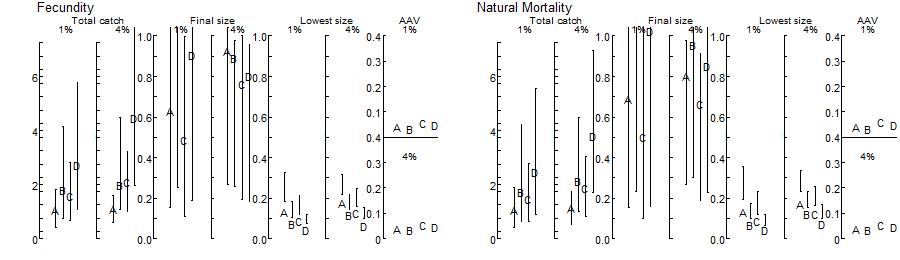
\includegraphics[]{SC66aRMP10_Part2_T20-D.jpeg}
\caption{
Zeh plots for trial T20
[Episodic events and survey bias = 1.5]
(A = 100-year current, B = 300-year current, C = 100-year alternate, and D = 300-year alternate)
when initial depletion is 99\%.
Results are shown when density-dependence impacts fecundity (left panel) and when it impacts natural mortality (right panel).
}
\end{figure}


% %%%%%%%%%%%%%%%%%%%%%%%%%%%%%%%%%%%%%%%%%%%%%%%%%%%%%%%%%%%%%%%%%%%%%%%%%%%%%%%
% %%%%%%%%%%%%%%%%%%%%%%%%%%%%%%%%%%%%%%%%%%%%%%%%%%%%%%%%%%%%%%%%%%%%%%%%%%%%%%%
% %%%% T21: Episodic events, survey bias 1.5 D,R,S, and CV = 0.2
% %%%%%%%%%%%%%%%%%%%%%%%%%%%%%%%%%%%%%%%%%%%%%%%%%%%%%%%%%%%%%%%%%%%%%%%%%%%%%%%
% %%%%%%%%%%%%%%%%%%%%%%%%%%%%%%%%%%%%%%%%%%%%%%%%%%%%%%%%%%%%%%%%%%%%%%%%%%%%%%%
% \phantomsection
% \stepcounter{section}
% \setcounter{figure}{0}
% <<echo = FALSE, include = FALSE>>=
% keep <- subset(sheet, depl %in% c(0.3) & T == "T21")
% if (NROW(keep) > 4) stop("Too many factors selected")
% plotnamea <- as.character(keep$name)[1]
% plotnamea <- paste(paper, substring(plotnamea, 4, nchar(plotnamea) - 1), sep = "_")
% depl <- formatC(keep$depl * 100, format = "f", digits = 0)[1]
% plot_curve(aep100, aep300, ps4100, ps4300, keep, plotnamea, part = 2)

% keep <- subset(sheet, depl %in% c(0.6) & T == "T21")
% if (NROW(keep) > 4) stop("Too many factors selected")
% plotnameb <- as.character(keep$name)[1]
% plotnameb <- paste(paper, substring(plotnameb, 4, nchar(plotnameb) - 1), sep = "_")
% depl[2] <- formatC(keep$depl * 100, format = "f", digits = 0)[1]
% plot_curve(aep100, aep300, ps4100, ps4300, keep, plotnameb, part = 2)
% @

% \begin{figure}[H]
% \centering
% \includegraphics[]{paste(plotnamea, "jpeg", sep = ".")}
% \includegraphics[]{paste(plotnameb, "jpeg", sep = ".")}
% \caption{
% Zeh plots for trial as.character(keep$T[1])
% [Episodic events, survey bias = keep$survbias[1], and CV = ?]
% (A = 100-year current, B = 300-year current, C = 100-year alternate, and D = 300-year alternate)
% when initial depletion is depl[1]\% (upper panel) and depl[2]\% (lower panel).
% Results are shown when density-dependence impacts fecundity (left panel) and when it impacts natural mortality (right panel).
% }
% \end{figure}

% <<echo = FALSE, include = FALSE>>=
% keep <- subset(sheet, depl %in% c(0.99) & T == "T21")
% if (NROW(keep) > 4) stop("Too many factors selected")
% plotnamea <- as.character(keep$name)[1]
% plotnamea <- paste(paper, substring(plotnamea, 4, nchar(plotnamea) - 1), sep = "_")
% depl <- formatC(keep$depl * 100, format = "f", digits = 0)[1]
% plot_curve(aep100, aep300, ps4100, ps4300, keep, plotnamea, part = 2)
% @

% \begin{figure}[H]
% \centering
% \includegraphics[]{paste(plotnamea, "jpeg", sep = ".")}
% \caption{
% Zeh plots for trial as.character(keep$T[1])
% [Episodic events and survey bias = keep$survbias[1]]
% (A = 100-year current, B = 300-year current, C = 100-year alternate, and D = 300-year alternate)
% when initial depletion is depl[1]\%.
% Results are shown when density-dependence impacts fecundity (left panel) and when it impacts natural mortality (right panel).
% }
% \end{figure}

\end{landscape}
\end{document}
